\documentclass[a4paper, british]{article}

\usepackage[utf8]{inputenc}
\usepackage[T1]{fontenc}
\usepackage{babel}
% \usepackage[margin=2.5cm,a4paper]{geometry}
% \usepackage[skip=1em]{parskip}
\usepackage{lmodern} 
\usepackage{microtype}
% \usepackage{xcolor}
\usepackage{graphicx}
\graphicspath{ {./figures/} }
% \usepackage{float}
% \usepackage{enumitem}
\usepackage{adjustbox} % rescale - useful for Dia exported TeX
\usepackage{tikz}
% \usepackage{pgfplots}
\usepackage{booktabs} %tables no vertical lines
% \usepackage{array}
% \usepackage{authblk}
% \usepackage{fancyhdr} %headers and footers
% \usepackage{titlesec}
% \usepackage{tcolorbox} % framed text boxes
% \usepackage{mathtools, amssymb, amsthm}
% \usepackage{gensymb}
\usepackage{chemformula} % chemical formulae
\usepackage{chemfig} % molecular figures
\usepackage{siunitx}
\usepackage{csquotes}
\usepackage[titletoc, title]{appendix}
% \usepackage{lettrine} % initials

\usepackage[
pdfauthor={Adam Menne},
pdftitle={Chemistry 254 - Practical 1},
pdfsubject={},
pdfkeywords={}]{hyperref}

\usepackage[noabbrev]{cleveref}

\usepackage[
backend=biber,
style=numeric,
sorting=none,
doi=true,
isbn=false
]{biblatex}
\addbibresource{citations.bib}

\setlength{\parskip}{1em}
\setlength{\parindent}{0em}
\linespread{1.3}

\title{Chemistry 254\\ Experiment 8\\ Thermodynamics of a chemical cell}
\date{Last editted on \today}
\author{Adam Menne\\ Stellenbosch University}

\begin{document}

\maketitle

\begin{abstract}
\noindent
In this practical the temperature dependence of cell potential in a chemical cell was investigated, with a focus on the thermodynamic properties responsible for this dependence.
\end{abstract}

\tableofcontents

\newpage

\section{Introduction}

In this practical we investigate the temperature dependence of \(emf\) in a standard button cell, by fitting a linear regression to empirical data. From the linear regression, we extract the necessary quantity to calculate various thermodynamic properties of the cell reaction.


\section{Results}

The fit on the linear regression has a percent error of 0.001543 and 4.994e-6 for the intercept and slope respectively. This indicates, atleast approximately, a linear relationship between \(emf\) and temperature. See \cref{fig:regression}

\begin{figure}[htb]
    \centering
    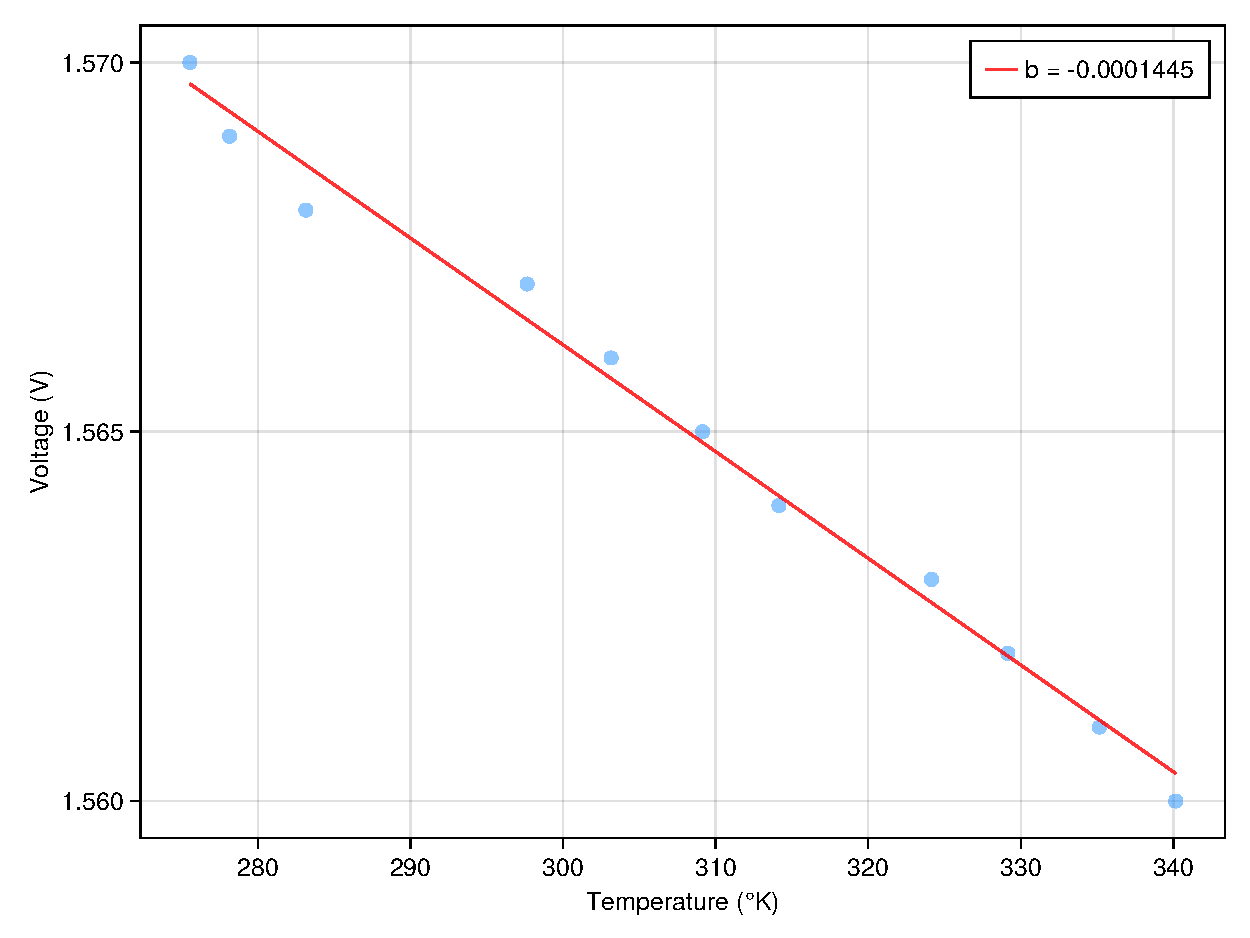
\includegraphics[width=\textwidth]{figures/regression.pdf}
    \caption{Voltage over temperature, with linear regression}
    \label{fig:regression}
\end{figure}

At room temperature (24.5 \textcelsius{}), the cell had an \(emf\) of 1.567 \((V)\), the predicted result from the linear regression is 1.5665\ldots \((V)\). The percent error is 0.03087. 

\begin{table}[htb]
    \centering
    \caption{Thermodynamic properties}
    \begin{tabular}{lcc}
        \addlinespace
        \toprule
        & Empirical & Standard\\ 
        \midrule
        \(\Delta H\ (kJ\ mol^{-1})\) & -308.4 & -319.4\\
        \(\Delta S\ (J\ K^{-1}\ mol^{-1})\) & -27.89 & -76.6\\
        \bottomrule
        \end{tabular}
        \label{table:data}   
\end{table}

Our empirical value for enthalpy matches well with known values for the cell reaction in question. However the value for entropy are less in line with the expected value. See \cref{table:data}

A static export of the notebook containing all analysis and figures is availible at \url{https://adammenne.github.io/chemistry_254/practical_1/plots.html}.\\ With full source code availble at \url{https://github.com/AdamMenne/chemistry_254/tree/master/practical_1}

\section{Discussion}

One alteration to the experimental procedure was made. Due to the limited resolution of the multimetres used, and the heated water bath not reaching the desired temperatures, the number of data points that were sampled were, if not inadequate, undesirable. To gather a larger number of data points, we exposed the cells to a larger temperature range by placing the oil bath in an ice-water slurry, allowing the cell to be cooled to a temperature of 2.4 \textcelsius{}, pushing the number of data points from 8 to 11.

The small value for percent error for \(emf\) at room temperature is a result of a few factors, partly as can be seen in \cref{fig:regression}, there is a periodic trend of datapoints being in clusters, the first three, and next two groups of four, all appear to express a perfectly linear relationship between \(emf\) and temperature. However these clusters are shifted relative to each other. This is likely due to rounding errors introduced by the multimetre. As such it is mostly coincidence that the datapoint at room temperature happens to lie almost perfectly on the regression line.

The mismatch between the expected and known value for entropy of the cell reaction, is the largest discrepancy in this report, and is in all likelyhood due to an error in calculation.

\end{document}